% Standalone vector rebuild of the "Relative-periodic domain selection by
% Bernoulli NML" 4-panel figure. Compile with pdflatex to produce
% winnower_nml_figure.pdf, which the late-breaking abstract includes.
\documentclass[border=6pt]{standalone}
\usepackage{tikz}
\usepackage{amsmath,amssymb}
\usetikzlibrary{positioning,arrows.meta,backgrounds,fit,calc}
\begin{document}
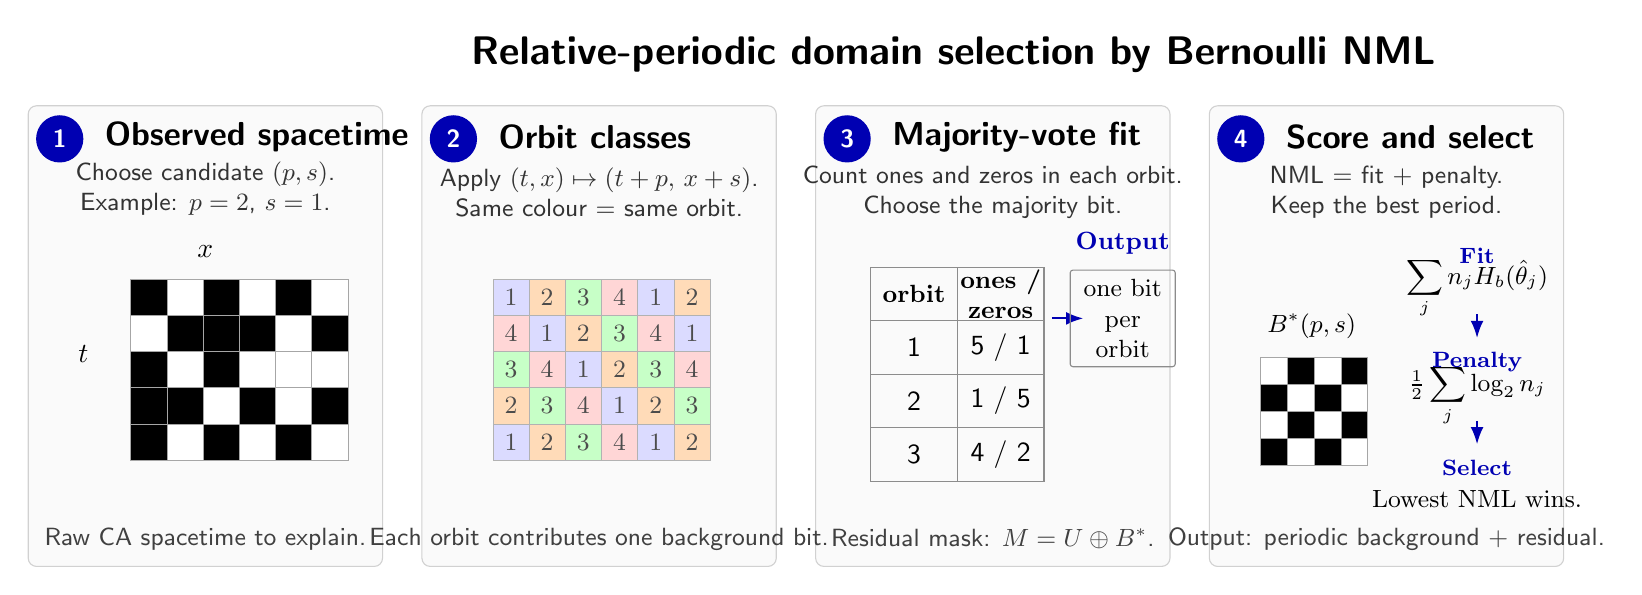
\begin{tikzpicture}[font=\sffamily]
\def\cs{0.46}            % grid cell size
\def\P{5.0}             % panel pitch
\tikzset{
  badge/.style={circle, fill=blue!70!black, text=white, inner sep=0pt,
    minimum size=6mm, font=\sffamily\bfseries\small},
  ptitle/.style={font=\sffamily\bfseries\large},
  pdesc/.style={font=\sffamily\small, align=center, text=black!80},
  pfoot/.style={font=\sffamily\small, align=center, text=black!75},
  arr/.style={-{Latex[length=2.2mm]}, thick, blue!70!black},
}

% ---- panel backgrounds ----
\foreach \i in {0,1,2,3}{
  \draw[rounded corners=3pt, fill=black!2, draw=black!18]
    ($(\i*\P-0.35, 0.7)$) rectangle ($(\i*\P+4.15, -5.15)$);
}

% =====================================================================
% Panel 1: Observed spacetime
% =====================================================================
\def\X{0}
\node[badge] at (\X+0.05,0.28) {1};
\node[ptitle, anchor=west] at (\X+0.5,0.3) {Observed spacetime};
\node[pdesc] at (\X+1.9,-0.35) {Choose candidate $(p,s)$.\\ Example: $p=2$, $s=1$.};
% axes labels
\node[font=\itshape] at (\X+1.9,-1.15) {$x$};
\node[font=\itshape] at (\X+0.35,-2.45) {$t$};
% U grid: checkerboard with three defects (residual)
\begin{scope}[shift={(\X+0.95,-1.5)}]
  \foreach \r in {0,...,4}{ \foreach \c in {0,...,5}{
      \pgfmathtruncatemacro{\v}{mod(\r+\c,2)}
      \pgfmathtruncatemacro{\dfct}{ ( (\r==1 && \c==2) || (\r==3 && \c==0) || (\r==2 && \c==4) ) ? 1 : 0 }
      \pgfmathtruncatemacro{\blk}{ \v==\dfct ? 1 : 0 } % checkerboard, flipped on defects
      \ifnum\blk=1\relax \def\col{black}\else \def\col{white}\fi
      \fill[\col] (\c*\cs,-\r*\cs) rectangle ++(\cs,-\cs);
      \draw[black!35, line width=0.2pt] (\c*\cs,-\r*\cs) rectangle ++(\cs,-\cs);
  }}
\end{scope}
\node[pfoot] at (\X+1.9,-4.8) {Raw CA spacetime to explain.};

% =====================================================================
% Panel 2: Orbit classes
% =====================================================================
\def\X{\P}
\node[badge] at (\X+0.05,0.28) {2};
\node[ptitle, anchor=west] at (\X+0.5,0.3) {Orbit classes};
\node[pdesc] at (\X+1.9,-0.4) {Apply $(t,x)\mapsto(t+p,\,x+s)$.\\ Same colour $=$ same orbit.};
\begin{scope}[shift={(\X+0.55,-1.5)}]
  \foreach \r in {0,...,4}{ \foreach \c in {0,...,5}{
      \pgfmathtruncatemacro{\val}{mod(\c-\r+8,4)+1}
      \ifcase\val\or\def\cc{blue!14}\or\def\cc{orange!28}\or\def\cc{green!22}\or\def\cc{red!16}\fi
      \fill[\cc] (\c*\cs,-\r*\cs) rectangle ++(\cs,-\cs);
      \draw[black!30, line width=0.2pt] (\c*\cs,-\r*\cs) rectangle ++(\cs,-\cs);
      \node[font=\small, text=black!70] at (\c*\cs+0.5*\cs,-\r*\cs-0.5*\cs) {\val};
  }}
\end{scope}
\node[pfoot] at (\X+1.9,-4.8) {Each orbit contributes one background bit.};

% =====================================================================
% Panel 3: Majority-vote fit
% =====================================================================
\def\X{2*\P}
\node[badge] at (\X+0.05,0.28) {3};
\node[ptitle, anchor=west] at (\X+0.5,0.3) {Majority-vote fit};
\node[pdesc] at (\X+1.9,-0.4) {Count ones and zeros in each orbit.\\ Choose the majority bit.};
% table
\begin{scope}[shift={(\X+0.35,-1.35)}]
  \draw[black!45] (0,0) rectangle (2.2,-2.72);
  \draw[black!45] (1.1,0) -- (1.1,-2.72);
  \draw[black!45] (0,-0.68) -- (2.2,-0.68);
  \draw[black!45] (0,-1.36) -- (2.2,-1.36);
  \draw[black!45] (0,-2.04) -- (2.2,-2.04);
  \node[font=\small\bfseries] at (0.55,-0.34) {orbit};
  \node[font=\small\bfseries, align=center] at (1.65,-0.34) {ones /\\ zeros};
  \node at (0.55,-1.02) {1}; \node at (1.65,-1.02) {5 / 1};
  \node at (0.55,-1.70) {2}; \node at (1.65,-1.70) {1 / 5};
  \node at (0.55,-2.38) {3}; \node at (1.65,-2.38) {4 / 2};
\end{scope}
% output box + arrow
\draw[arr] (\X+2.65,-2.0) -- (\X+3.05,-2.0);
\node[draw=black!45, rounded corners=1pt, align=center, font=\small,
      minimum height=0.95cm, text width=1.1cm] at (\X+3.55,-2.0) {one bit\\ per orbit};
\node[font=\small\bfseries, text=blue!70!black] at (\X+3.55,-1.05) {Output};
\node[pfoot] at (\X+1.9,-4.8) {Residual mask: $M = U \oplus B^{*}$.};

% =====================================================================
% Panel 4: Score and select
% =====================================================================
\def\X{3*\P}
\node[badge] at (\X+0.05,0.28) {4};
\node[ptitle, anchor=west] at (\X+0.5,0.3) {Score and select};
\node[pdesc] at (\X+1.9,-0.4) {NML $=$ fit $+$ penalty.\\ Keep the best period.};
% B* grid (clean checkerboard), 4x4, on the left, vertically centred
\begin{scope}[shift={(\X+0.3,-2.5)}]
  \def\bcs{0.34}
  \foreach \r in {0,...,3}{ \foreach \c in {0,...,3}{
      \pgfmathtruncatemacro{\v}{mod(\r+\c,2)}
      \ifnum\v=1\relax \def\col{black}\else \def\col{white}\fi
      \fill[\col] (\c*\bcs,-\r*\bcs) rectangle ++(\bcs,-\bcs);
      \draw[black!35, line width=0.2pt] (\c*\bcs,-\r*\bcs) rectangle ++(\bcs,-\bcs);
  }}
\end{scope}
\node[font=\small] at (\X+0.95,-2.1) {$B^{*}(p,s)$};
% score stack on the right: label above formula, centred, no overlap
\node[font=\footnotesize\bfseries, text=blue!70!black] at (\X+3.05,-1.2) {Fit};
\node[font=\small] at (\X+3.05,-1.62) {$\displaystyle\sum_j n_j H_b(\hat\theta_j)$};
\draw[arr] (\X+3.05,-1.95) -- (\X+3.05,-2.25);
\node[font=\footnotesize\bfseries, text=blue!70!black] at (\X+3.05,-2.55) {Penalty};
\node[font=\small] at (\X+3.05,-2.98) {$\displaystyle\tfrac{1}{2}\sum_j \log_2 n_j$};
\draw[arr] (\X+3.05,-3.3) -- (\X+3.05,-3.6);
\node[font=\footnotesize\bfseries, text=blue!70!black] at (\X+3.05,-3.9) {Select};
\node[font=\small] at (\X+3.05,-4.3) {Lowest NML wins.};
\node[pfoot] at (\X+1.9,-4.8) {Output: periodic background $+$ residual.};

% =====================================================================
% Title
% =====================================================================
\node[font=\sffamily\bfseries\Large] at (2*\P-0.5+1.9,1.35)
  {Relative-periodic domain selection by Bernoulli NML};

\end{tikzpicture}
\end{document}
